%; whizzy chapter -dvi
% -initex iniptex -latex platex -format platex -bibtex jbibtex -fmt fmt
% 以上 whizzytex を使用する場合の設定。
 
%     Tokyo Debian Meeting resources
%     Copyright (C) 2012 Junichi Uekawa
%     Copyright (C) 2011, 2015 Nobuhiro Iwamatsu

%     This program is free software; you can redistribute it and/or modify
%     it under the terms of the GNU General Public License as published by
%     the Free Software Foundation; either version 2 of the License, or
%     (at your option) any later version.

%     This program is distributed in the hope that it will be useful,
%     but WITHOUT ANY WARRANTY; without even the implied warranty of
%     MERCHANTABILITY or FITNESS FOR A PARTICULAR PURPOSE.  See the
%     GNU General Public License for more details.

%     You should have received a copy of the GNU General Public License
%     along with this program; if not, write to the Free Software
%     Foundation, Inc., 51 Franklin St, Fifth Floor, Boston, MA  02110-1301 USA

%  preview (shell-command (concat "evince " (replace-regexp-in-string "tex$" "pdf"(buffer-file-name)) "&"))

%%ここからヘッダ開始。

\documentclass[mingoth,a4paper]{jsarticle}
\usepackage{monthlyreport}
% 日付を定義する、毎月変わります。
\newcommand{\debmtgyear}{2015}
\newcommand{\debmtgmonth}{6}
\newcommand{\debmtgdate}{20}
% started from zero:
% (let ((year 2013) (month 7)) (+ (* (- year 2005) 12) month -1))
\newcommand{\debmtgnumber}{127}

\begin{document}

\begin{titlepage}
\thispagestyle{empty}
% タイトルページ:編集必要な部分は最初のマクロに飛ばすこと

\vspace*{-2cm}
第\debmtgnumber{}回 東京エリア Debian 勉強会資料\\
\hspace*{-2cm}

\includegraphics{image2012-natsu/dotdeb.pdf}\\
\hfill{}\debmtgyear{}年\debmtgmonth{}月\debmtgdate{}日

% ここはアップデートすること
% 全角文字にしないとフォントのサイズが合わないので注意
\rotatebox{10}{\fontsize{30}{30} {\gt 特集:Debianと脆弱性対応}}\\

\vspace*{-2cm}
\hfill{}
\includegraphics[height=6cm]{image200502/openlogo-nd.eps}
\end{titlepage}

\newpage

\begin{minipage}[b]{0.2\hsize}
 \definecolor{titleback}{gray}{0.9}
 \colorbox{titleback}{\rotatebox{90}{\fontsize{80}{80} {\gt デビアン勉強会} }}
\end{minipage}
\begin{minipage}[b]{0.8\hsize}
\hrule
\vspace{2mm}
\hrule
\begin{multicols}{2}
\tableofcontents
\end{multicols}
\vspace{2mm}
\hrule
\end{minipage}

\dancersection{事前課題}{野島 貴英}

今回の事前課題は以下です:
\begin{enumerate}
\item 本日、何の作業をやるかを宣言ください。
\item (オプション) どこで今回の勉強会の開催を知りましたか?
\item (オプション) 何について聞きたい/参加者と話をしたいですか?
\end{enumerate}
この課題に対して提出いただいた内容は以下です。
\begin{multicols}{2}
{\small
\begin{prework}{ 野島 }
  \begin{enumerate}
  \item Q.hack timeに何をしますか?\\
    A. Nook HD+をそろそろdebianを動かす件かな?
  \item (オプション)Q.何について聞きたい/参加者と話をしたいですか?\\
    A. Debian! Debian! Debian!
  \end{enumerate}
\end{prework}

\begin{prework}{ pike }
  \begin{enumerate}
  \item Q.hack timeに何をしますか?\\
    A. Debian 関連ドキュメント読書
  \item (オプション)Q.どこで今回の勉強会の開催を知りましたか?\\
    A. その他
  \end{enumerate}
\end{prework}

\begin{prework}{ wskoka }
  \begin{enumerate}
  \item Q.hack timeに何をしますか?\\
    A. mipsやtileへの移植
  \item (オプション)Q.どこで今回の勉強会の開催を知りましたか?\\
    A. その他
  \end{enumerate}
\end{prework}

\begin{prework}{ dictoss }
  \begin{enumerate}
  \item Q.hack timeに何をしますか?\\
    A. OSC2015北海道のブース出展のまとめ、pptp-linuxパッケージのkfreebsd対応
  \item (オプション)Q.どこで今回の勉強会の開催を知りましたか?\\
    A. Debian JPのメーリングリスト
  \end{enumerate}
\end{prework}

\begin{prework}{ issei }
  \begin{enumerate}
  \item Q.hack timeに何をしますか?\\
    A. 個人で作ってるプログラムの開発を進めたいです。
  \item (オプション)Q.どこで今回の勉強会の開催を知りましたか?\\
    A. その他
  \end{enumerate}
\end{prework}

\begin{prework}{Roger Shimizu}
  \begin{enumerate}
  \item Q.hack timeに何をしますか?\\
    A. Debian BTSの勉強
  \item (オプション)Q.どこで今回の勉強会の開催を知りましたか?\\
    A. Twitter (@tokyodebian)
  \end{enumerate}
\end{prework}


}
\end{multicols}

\dancersection{Debian Trivia Quiz}{野島 貴英}

 Debianの昨今の話題についてのQuizです。

今回の出題範囲は\url{debian-devel-announce@lists.debian.org} や \url{debian-news@lists.debian.org}に投稿された
内容などからです。

\begin{multicols}{2}
%; whizzy-master ../debianmeetingresume201311.tex
% $B0J>e$N@_Dj$r$7$F$$$k$?$a!"$3$N%U%!%$%k$G(B M-x whizzytex $B$9$k$H!"(Bwhizzytex$B$,MxMQ$G$-$^$9!#(B
%

\santaku
{Debian 8.1 $B$,%j%j!<%9$5$l$^$7$?!#$$$D$@$C$?$G$7$g$&$+!)(B}
{2015/6/6}
{2015/6/13}
{2015/6/20}
{A}
{$B$$$/$D$+$N@H<e@-BP:v$d!"%P%0%U%#%C%/%9$,9T$o$l$?%Q%C%1!<%8$,<h$j9~$^$l$^$7$?!#(BDebian 8(Jessie)$B$r%$%s%9%H!<%k$7$?$P$+$j$N?M$O!"AaB.%"%C%W%0%l!<%I$7$^$7$g$&!*(B}

\santaku
{2015/6/10$B$K$F!"(Bunstable$BHG$N%=!<%9%Q%C%1!<%8$N?t$O$$$/$D$K$J$C$?$G$7$g$&$+!)(B}
{21,000}
{22,000}
{23,000}
{B}
{$B?k$K(B22,000$B$rD6$($?$=$&$G$9!#%P%$%J%j%Q%C%1!<%8$N?t$O(B45,542$B$H$N;v!#1W!9A}$($F$$$/$h$&$G$9!#(B}

\santaku
{AutomaticDebugPackages$B$NDs0F$H$O2?!)(B}
{$BBgE}0l(BDebian$B$N4d>>$5$s$N%G%P%C%0%Q%C%1!<%8$N7o$r<B;\$9$k(B}
{$B<+F0$G%G%P%C%0=PMh$k$h$&$K$9$k(B}
{-dbg$B%Q%C%1!<%8$r;_$a!"(B.ddeb$B%Q%C%1!<%8$r:n$k(B}
{C}
{$B:#$^$G!"%G%P%C%0%7%s%\%k$O(B-dbg$B%Q%C%1!<%8$GG[I[$5$l$F$$$^$7$?!#$7$+$7$J$,$i!"$3$A$i$N(B-dbg$B%Q%C%1!<%8$OB>$N%G%P%C%0$H$O2?$i4X78$N$J$$%Q%C%1!<%8$H0l=o$K(Bmirror$B$5$l$k$?$a!"(B-dbg$B%Q%C%1!<%8$NMxMQ<T$,$H$F$b>/$J$$$K$b$+$+$o$i$:!"(Bmirror$B@h$N;q8;$r$=$NJ,>CHq$7$F$7$^$$$^$9!#:#2s$NDs0F$O!"%G%P%C%0%7%s%\%k(B.ddeb$B$H$$$&%Q%C%1!<%8$K$7$F$7$^$$!"$3$A$i$N%Q%C%1!<%8$K$D$$$F$O(Bmirror$B@h$b8:$i$9!J$7$J$$!)!K$H$$$&;v$r8!F$$9$k$b$N$G$9!#(B}





\end{multicols}

\dancersection{最近のDebian関連のミーティング報告}{野島 貴英}

\subsection{第126回東京エリアDebian勉強会}

\begin{itemize}
\item 場所はスクウェア・エニックスさんのセミナルームをお借りしての開催でした。
\item 参加者は6名でした。
\item セミナ内容は野首さんによる「自然言語処理チーム(pkg-nlp-ja)とパッケージ」でした。
\item 残りの時間でhack timeを行い、成果発表をしました。
\item 宴会の代わりに、「まいどおおきに食堂」で夕食会をやりました。  
\end{itemize} 

  セミナは野首さん(Debian公式開発者)による、自然言語処理プログラムの動作に纏わるいろいろなお話を聞かせていただきました。自然言語処理の基礎になっている、辞書のデータ構造、アルゴリズムについての紹介が主な内容でした。普段、自然言語処理の詳細に触れることが無い人にとっては、非常に新鮮な内容だったと思います。
  
 何気ない日本語の処理をDebianで行う場合でも、こういったプログラムの力を借りる事も多いと思います。自然言語処理のパッケージの処理、重要さについて、より広く知られるようになると良いと思いました。
 
% % (query-replace-regexp "<.*?>" "")
% % (query-replace-regexp "^[	 ]\+" "")

%-------------------------------------------------------------------------------
\dancersection{Debianと脆弱性対応のあれこれをまとめてみた}{野島 貴英}
%-------------------------------------------------------------------------------

\subsection{はじめに}

 コンピュータセキュリティの勉強会にて登壇を頼まれました。ちょうど良かったので、Debianの脆弱性対応をおさらいして、発表してみることにします。

\subsection{Debianのセキュリティチーム}

 Debianパッケージの脆弱性問題を専門に扱っている心臓部のチームの連絡先は以下の通りです。

\begin{itemize}
\item security@debian.org または 
\item team@security.debian.org
\end{itemize}

\subsection{脆弱性に関するML}

 Debianの脆弱性に関するアナウンス・議論が行われているMLは次のとおりです。

 \begin{itemize}
 \item  Debianパッケージのセキュリティに関するアナウンス\\
debian-security-announce@lists.debian.org\\
アーカイブ:\\
\url{https://lists.debian.org/debian-security-announce/}
 \item  Debianパッケージの脆弱性に関するオープンな議論\\
debian-security@lists.debian.org\\
アーカイブ:\url{https://lists.debian.org/debian-security/}
 \end{itemize}

\subsection{脆弱性対応が行われないアーカイブエリア}

 Debianパッケージ群は、main/contrib/non-freeのアーカイブエリアでそれぞれ提供されています。実は、脆弱性対応について、contrib/non-freeのアーカイブエリアのパッケージについては、基本的に除外されています。

 こちらの理由としては、contribとnon-freeに収められたソフトウェアのライセンスの問題によります。これらのソフトウェアはライセンスの都合上、勝手に直すことが許諾されていない場合があるためとなります。もちろん、contribとnon-freeであっても、ライセンス上、直しても良いものもあり、こちらについては通常の通りセキュリティチームにて脆弱性対応が図られることがあります。

\subsection{脆弱性に関しての対応の流れ}

 DebianユーザあるいはDebianの関係者にかかわらず、もし脆弱性の問題を見つけたら、
\begin{description}
\item [PAT1:] 既知の問題(公開済脆弱性情報)の場合は、securityタグをつけてBTSしてください。
\item [PAT2:] 既知でない場合は、そっとsecurity@debian.org またはteam@security.debian.org にメールで連絡(英文)し、あとは指示に従えば良いです。
\end{description}

 もちろん、脆弱性対策パッチも書いたのであれば、報告の際にパッチも一緒に送ると喜ばれます。

\subsubsection{既知の脆弱性でない場合の動き}

 既知の脆弱性でない場合、セキュリティチームはDebian以外のベンダ(ディストリビューション等含む)関係者らにも脆弱性情報が共有され、CVEなどの脆弱性情報データベース登録にも協力する動きが取られます。

\subsubsection{既知の脆弱性の収集}

 Mitre社(CVEのDBを管理している会社)から、CVEの情報を定期的に取り込んでいます。こちらの情報に基づき、Debianに関係ある・なし、重要度を判定して仕分けされ、バグ追跡システムに登録していく仕組み(インフラ)があります。

\subsection{脆弱性対応状況の確認方法}

 以下のサイトで状況を確認できます。

 \begin{enumerate}
\item セキュリティ観点から確認したい場合
  \begin{itemize}
  \item \url{https://security-tracker.debian.org/tracker/}
  \item 様々な視点から、巷の脆弱性データベースとDebianの各パッケージの対応状況を確認可能です。
  \end{itemize}
\item QA観点から確認したい場合
  \begin{itemize}
  \item \url{https://tracker.debian.org/}
     \item Debianパッケージについて、現在のバグの修正状況、パッケージのリリース状況がパッケージ毎にわかります。
  \end{itemize}
\item BTSした・されたものを確認したい場合
  \begin{itemize}
  \item \url{https://bugs.debian.org/}
  \item BTSした結果がどう扱われているか、進行しているか確認できます。
  \end{itemize}  
\end{enumerate}

 \subsection{その他トピック}

 以上で、まとめとしては終わったので、昨今のDebianのセキュリティに関するトピックをいくつか紹介します。

 \subsubsection{hardening}

  C/C++で書かれたプログラムについて、gccの機能を活用して、セキュリティ強化を行ったDebianパッケージを作る試みです。hardening有効時、ビルド時に実際に付け加えられるgccのオプションは以下の通りです。
  
\begin{commandline}
-fstack-protector-strong -Wformat -Werror=format-security -D_FORTIFY_SOURCE=2
\end{commandline}

 \subsubsection{Debianパッケージ済みの脆弱性静的解析ツール群}

  Debianでパッケージ済の脆弱性静的解析ツール群があります。

\begin{table}
\begin{center}
\begin{tabular}{|c|c|p{5cm}|}
\hline
項番 & パッケージ名 & 概要 \\ \hline \hline
1 & flawfinder & C/C++にてセキュリティ上問題の起きそうな部分を指摘。 \\ \hline
2 & rats & C, Perl, PHP, Pythonのコード上問題の起きそうな部分を指摘。\\ \hline
3 & pscan & C/C++にてformat文の文字列について問題の起きそうな部分を指摘。 \\ \hline
\end{tabular}
\end{center}
\caption{Debianパッケージ済み脆弱性静的解析ツール}
\end{table}

\subsubsection{lintian}

 lintianは、Debianパッケージについて、自動でスキャンして問題点を解析して警告してくれるツールであり、ある程度のセキュリティ対策の為の対応がパッケージ開発にあたり必須になっており、こちらが過不足なく行われているかをスキャンして開発者に教えてくれます。

 昨今にて搭載されたセキュリテイ対応の例として、梱包されているドキュメントにHTMLソースがあった場合、外部リンクが含まれているかをスキャンする事が追加されました。これは、もし、パッケージに含まれるドキュメントがHTMLであった場合に、外部リンクへアクセスするようなタグが混ざっているような事が無いようにします。もし、そういったタグやリンクが残っていると、ドキュメントをブラウザで開いた時に、うっかり悪意のあるサイトへ自動的に誘導されてしまうのを防ぎます。

\subsubsection{systemd}

 systemdにはセキュリティに関して強化を図ることが出来るオプションがいくつもあります。こちらをどう活かして、systemdの*.serviceファイルを作るかというお話です。
 
 良い文章として、「Security Features in systemd」\url{http://0pointer.net/public/systemd-nluug-2014.pdf}がありますので、見てみるとよいでしょう。

\subsubsection{Reproducible Builds}

 Debianの22,000を超えるソースパッケージを一旦再ビルドし、すでに配布されているDebianパッケージのバイナリと照合する試みの事です。こちらにより、Debianパッケージにいつの間にか悪意のあるバイナリが含まれているような事が無いかをチェックするのが狙いです。Debianの他にも、Fedora/OpenSUSE/NixOSでも行われているとのことです。

 詳しくは、
 \begin{description}
\item [Debian]
  \url{http://reproducible.alioth.debian.org/presentations/2014-02-01-FOSDEM14.pdf}

\item [Fedora]
   \url{http://securityblog.redhat.com/2013/09/18/reproducible-builds-for-fedora/}
 \end{description}

を参照ください。
   
\subsubsection{LTS(Long Time Support)}

Debianの各バージョンについて、セキュリティアップデートについてのサポート切れまでの期間を3年→5年へ延長する試みです。但し、数万もあるソフトウェア全部について5年もサポートするのは非現実的なので、限られたパッケージのセキュリティアップデートのみ延長します。

\begin{figure}[H]
\begin{center}
 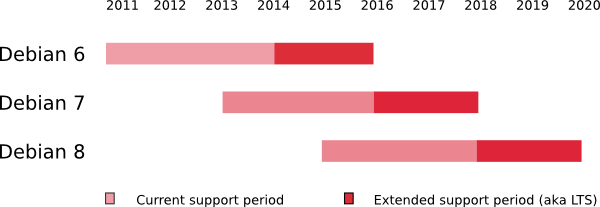
\includegraphics[width=0.7\hsize]{image201506/debian-lts-periods.png}
\end{center}
\caption{LTSのサポート期間}
\end{figure}

 LTSは無料でも利用できる一方、有償サポート契約も用意されています。Freexian社と有償サポート契約を行うのですが、払った値段に応じて、サポートしてくれるパッケージの選択の要望が通りやすくなるという特典があるようです。日本の会社にて契約締結実績はGREE社があります。

 有償サポート契約について詳しくは「Debian Long Term Support」\url{https://www.freexian.com/en/services/debian-lts.html}を参照ください。

\subsubsection{debian-security-supportパッケージ}

 debian-security-supportパッケージを導入し、check-support-statusコマンドを実行すると、
現在お使いのDebian機に導入されいているパッケージの脆弱性のサポートについて、サポート切れ、もしくは、何らかの理由により脆弱性対策にあたり制限を加えざるを得なかったもののリストが取れるようになりました。

 このコマンドの動作としては、
\begin{itemize}
\item  /usr/share/debian-security-support/security-support-ended
\item /usr/share/debian-security-support/security-support-limited
\end{itemize}
に記載されたパッケージのサポート状況に関する制限の情報と、実際に導入されていてるパッケージ名を照合することにより動作します。もし、これらのファイルから、制限があるパッケージがマシンに見つかった場合は、警告を出してくれます。なお、LTSでは、どこまでパッケージについて、脆弱性対応のサポートがなされているかの確認ができます。

\subsection{おわりに}

 Debianの脆弱性対応についてまとめてみました。Debianのセキュリティ維持の為、様々な努力が払われていることがわかりました。
   
%-------------------------------------------------------------------------------
\dancersection{会場での無線LANのつなぎ方}{野島 貴英,Roger}
%-------------------------------------------------------------------------------
 \subsection{はじめに}

 今回試験として、会場側でフィルタ無しのグローバル回線を用意しました。
ただ、会場側のセキュリティポリシーにより、wpa-psk AES hidden SSIDという
方式での提供となります。

 以下にDebianマシンでの接続方法を記載します。

 また、自分の環境では違うやり方でつながったという方は、野島まで
教えて下さい。こちらでもノウハウとして溜めていく予定です。

 \subsection{wpasupplicant及び/etc/network/interfacesを利用の場合}

 もっとも良いマニュアルは、/usr/share/doc/wpasupplicant/README.Debian.gz
となります。困った場合はこちらも合わせてご参照下さい。

 以下に/etc/network/interfacesの定義について会場の例を記載します。

\begin{commandline}
$ sudo vi /etc/network/interfaces
-----以下のエントリがなければ追記ここから----------
iface wlan0_debian inet dhcp
     wpa-conf /etc/wpa_supplicant/wpa_supplicant_debian.conf
-----以下のエントリがなければ追記ここまで----------
$ sudo vi /etc/wpa_supplicant/wpa_supplicant_debian.conf
-----以下のエントリを追記ここから----------
network={
     ssid=<<会場のSSID>>
     psk=<<会場のパスワード>>
     scan_ssid=1
}
-----以下のエントリを追記ここまで----------
$ sudo chmod 600 /etc/wpa_supplicant/wpa_supplicant_debian.conf
$ sudo ifup wlan0=wlan0_debian
\end{commandline}
%$

 また、ハマってしまった時のデバッグ方法は、
/usr/share/doc/wpasupplicant/README.Debian.gz中の''4. Trubleshooting''の章が便利です。

 \subsection{その他の無線LAN用パッケージを利用の場合}

 すみません、自分が情報を持たないため、現場で教えて下さい。

\cleartooddpage

\vspace*{15cm}
\hrule
\vspace{2mm}

\includegraphics[width=2cm]{image200502/openlogo-nd.eps}
\noindent \Large \bf Debian 勉強会資料\\
\noindent \normalfont \debmtgyear{}年\debmtgmonth{}月\debmtgdate{}日 \hspace{5mm}  初版第1刷発行\\
\noindent \normalfont 東京エリア Debian 勉強会 (編集・印刷・発行)\\
\hrule

\end{document}
